\documentclass[10pt,a4paper]{article}
\usepackage[utf8]{inputenc}
\usepackage[T1]{fontenc}
\usepackage{lmodern}
\usepackage[margin=1.5cm, top=1.4cm, bottom=1.4cm]{geometry}
\usepackage{hyperref}
\usepackage{enumitem}
\usepackage{titlesec}
\usepackage{xcolor}
\usepackage{graphicx}

\definecolor{accent}{HTML}{00686E}
\hypersetup{colorlinks=true, urlcolor=accent, linkcolor=accent}
\pagenumbering{arabic}
\setlength{\parindent}{0pt}

\titleformat{\section}{\large\bfseries\color{accent}}{}{0em}{}[\vspace{-0.6em}\rule{\textwidth}{0.8pt}]
\titlespacing{\section}{0pt}{7pt}{4pt}

\newcommand{\role}[4]{%
  \textbf{#1} \hfill \textbf{#2}\\[1pt]%
  \textit{#3} \hfill \textit{#4}\\[2pt]%
}
\setlist[itemize]{leftmargin=1.2em, itemsep=1.5pt, topsep=2pt, parsep=0pt}

\begin{document}

% ================= HEADER =================
\begin{minipage}[c]{0.80\textwidth}
  {\Huge\bfseries Prabhavit Gupta}\\[3pt]
  {\color{accent}\large Quality Engineer (Automation \& AI): Playwright, Claude Code \& Agentic Testing}\\[6pt]
  {\footnotesize +39 351 610 7807 ~$\vert$~
  \href{mailto:prabhavitg@gmail.com}{prabhavitg@gmail.com} ~$\vert$~
  \href{https://www.linkedin.com/in/prabhavit/}{linkedin.com/in/prabhavit} ~$\vert$~
  \href{https://github.com/prab-gupta}{github.com/prab-gupta} ~$\vert$~
  Venice, Italy (CET Time Zone / EU Permanent Resident)}
\end{minipage}\hfill
\begin{minipage}[c]{0.18\textwidth}
  \raggedleft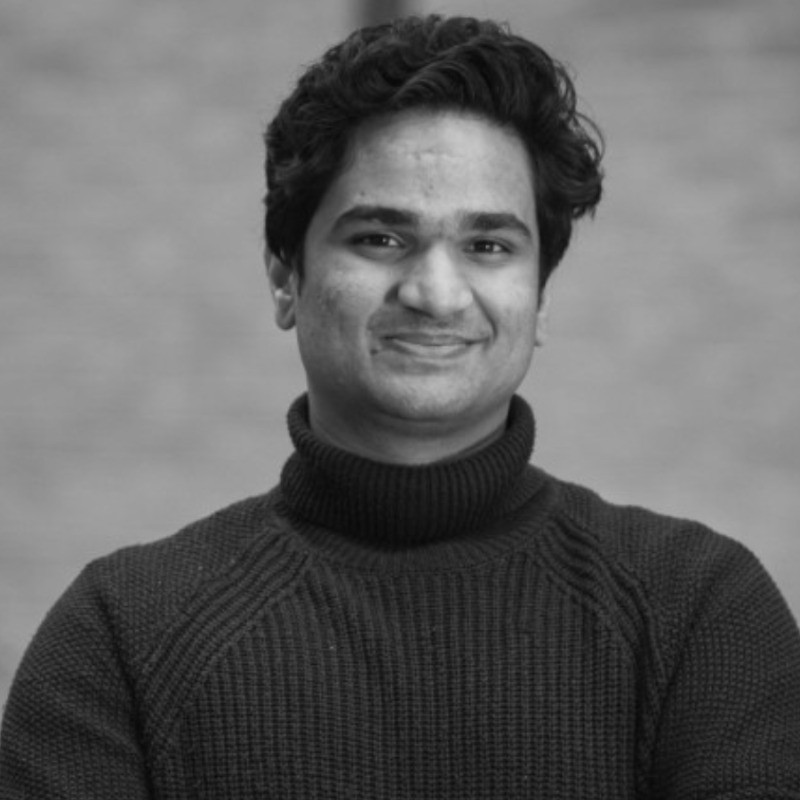
\includegraphics[width=2.0cm]{photo.jpg}
\end{minipage}
\vspace{-2pt}

% ================= SUMMARY =================
\section{Summary}
Quality Engineer and Systems Builder with 3 years of commercial production experience architecting automation-first testing frameworks, AI-native development workflows, and resilient web extraction pipelines. Deep practical expertise using Claude Code and AI coding assistants as primary accelerators to generate, maintain, and refactor automated Playwright test suites. Proven track record designing risk-based test strategies, embedding continuous quality gates into GitHub Actions CI/CD pipelines, and establishing agentic evaluation harnesses. Based in Venice, Italy (CET time zone) with an EU Long-Term Residence Permit (permanent unrestricted EU work authorization, no sponsorship required); available immediately for full-time remote roles.

% ================= TECHNICAL EXPERTISE =================
\section{Technical Expertise}
\begin{itemize}
  \item \textbf{Test Automation \& Frameworks:} Playwright (E2E, API testing, trace recording, parallel test workers, page object models), Jest, automated regression suites, risk-based test strategy design.
  \item \textbf{AI-Native Quality Engineering:} Claude Code workflows, agentic test generation, Model Context Protocol (MCP) integrations, LLM evaluation harnesses, self-healing test automation patterns.
  \item \textbf{Programming \& Scripting:} TypeScript, JavaScript (Node.js), Python3 (pytest, asyncio, requests), SQL (PostgreSQL), HTML5, DOM traversal, CSS/XPath locator strategies.
  \item \textbf{CI/CD \& Quality Gates:} GitHub Actions, automated regression test runs, PR blocking gates, Docker containerization, distributed logging, latency and error tracing.
  \item \textbf{Web Extraction \& Data Verification:} Automated DOM parsing, data schema enforcement, anomaly detection, HTTP mock servers, headless browser cluster management.
  \item \textbf{Languages \& Authorization:} English (C1 Professional, fluent), Hindi (Native), Italian (Conversational). EU Long-Term Residence Permit (unrestricted EU work authorization across all EU member states, no sponsorship required).
\end{itemize}

% ================= EXPERIENCE =================
\section{Experience}

\role{\href{https://flowspace.co}{FlowSpace.co}}{Mar 2024 - Aug 2026}{Lead Developer \& Quality Automation Engineer}{London, UK (remote)}
\begin{itemize}
  \item Architected and maintained the automated testing infrastructure using Playwright and TypeScript for a marketplace platform serving 4,500+ active enterprise users across Europe.
  \item Employed Claude Code and agentic workflows to rapidly author, scale, and maintain automated test coverage across critical user flows and API integrations.
  \item Embedded automated regression and contract test suites into GitHub Actions CI/CD pipelines, blocking failing pull requests and ensuring 99.8\% production reliability.
  \item Built automated evaluation harnesses to test tool-calling accuracy, retrieval grounding, and response consistency across multi-step AI features.
  \item Designed automated web extraction and monitoring routines verifying third-party data synchronization pipelines and flagging schema regressions in real time.
\end{itemize}

\role{Urlink}{Apr 2025 - Jul 2025}{Project Manager \& Solutions Developer (Freelance)}{Barcelona, Spain (remote)}
\begin{itemize}
  \item Designed risk-based test matrices and automated validation checks for custom full-stack web applications and data processing pipelines.
  \item Automated end-to-end user journeys and REST API endpoints using Playwright and Postman, ensuring seamless payment and database transactions.
  \item Partnered with client engineering squads to define acceptance criteria, isolate edge-case regressions, and accelerate release cycles.
\end{itemize}

\role{Independent Technical Consultant}{Aug 2023 - Feb 2024}{Software \& Automation Developer}{Venice, Italy}
\begin{itemize}
  \item Developed automated test scripts and validation tools for client web applications and ETL data extraction workflows using Python and Playwright.
  \item Built automated regression suites verifying database integrity and event-driven webhook delivery across integration endpoints.
  \item Authored quality engineering documentation, test plans, and automated setup scripts for client teams.
\end{itemize}

% ================= EDUCATION =================
\section{Education}
\role{Ca' Foscari University of Venice}{2020 - 2024}{BA in Philosophy, International Studies and Economics}{Venice, Italy}
\begin{itemize}
  \item Rigorous training in formal logic, analytical problem solving, systems analysis, and macroeconomic decision models.
\end{itemize}

\end{document}
